% \documentclass{report}

% \usepackage[ english, greek]{babel}
% \usepackage[utf8]{inputenc}
% \usepackage[LGR, T1]{fontenc}

% % % 

% \newcommand{\tl}{\textlatin}
% \newcommand{\en}{\selectlanguage{english}}
% \newcommand{\gr}{\selectlanguage{greek}}

% \usepackage{hyperref}  % package for linking figures etc
% \usepackage{enumitem}  % package for description with bullets
% \usepackage{graphicx}  % package for importing images
% \usepackage{mathtools} % package for math equation
% \usepackage{mathrsfs}  % package for math font
% \usepackage{indentfirst} % package for getting ident after section or paragraph
% \usepackage{subcaption} % package for subfigures
% \usepackage[export]{adjustbox}
% \usepackage{longtable} % package for multi pages tables
% \usepackage{multirow}  % package for tables, multirow
% \usepackage{amssymb}
% \usepackage{esvect}
% \usepackage[
% backend=bibtex,
% citestyle=authoryear,
% % citestyle=authoryear-comp,
% % citestyle=authoryear-ibid,
% bibstyle=numeric,
% sorting=ynt,
% % style=numeric,
% % style=alphabetic ,
% ]{biblatex}
% \addbibresource{References}

% \graphicspath{ {./theory/figures/} }       % path for images

% \begin{document}
\gr 
 
\chapter{\gr Στάδιο Ταξινόμησης\gr }
Στα προηγούμενα 2 κεφάλαια παρουσιάσαμε την διαδικασία που χρησιμοποιούμε για να δημιουργήσουμε
υποψήφια \en action tubes\gr,  τα οποία πιθανώς να περιέχουν κάποια πραγματοποιούμενη δράση ή μπορεί και όχι.
Τις περισσότερες φορές τα προτεινόμενα \en action tubes \gr ανήκουν στο φόντο, και γι' αυτό, όπως αναφέρθηκε
και στον προηγούμενο κεφάλαιο, είναι σημαντικό να επιλέξουμε έναν καλό αλγόριθμο που προτείνει καλές ακολουθίες
από πλαίσια. Ωστόσο, είναι αρκετά σημαντικό να επιλέξουμε και τον κατάλληλο ταξινομητή ο οποίος θα είναι σε θέση
με μεγάλη ακρίβεια να προβλέψει αν ένα υποψήφιο \en action tube \gr ανήκει σε μια γνωστή κατηγορία από δράσεις ή
ανήκει στο φόντο. Κι αυτό γιατί μπορεί να παράγουμε καλές προτάσεις για υποψήφιες δράσεις, αλλά αν ο ταξινομητής μας
δεν λειτουργεί στο έπακρο, το σύστημα μας πάλι θα αποτυγχάνει να αναγνωρίσει πραγματοποιούμενες δράσεις. \par
Η σωστή επιλογή ενός ταξινομητή είναι μια μεγάλη απόφαση που καλούμαστε να πάρουμε. Ωστόσο,  αυτός ο ταξινομητής θα δεχθεί
ορισμένους χάρτες ενεργοποίησης τους οποίους θα κληθεί να ταξινομήσει. Συνεπώς, εκτός από την καλή επιλογή ταξινομητή, εξίσου
σημαντική είναι η καλή επιλογή χαρακτηριστικών. Τέλος, μεγάλο ρόλο παίζει και η διαδικασία εκπαίδευσης του ταξινομητή προκειμένου
να είναι σε θέση να γενικεύει και καταστάσεις \en overfitting \gr να αποφεύγονται. \par
Σε αυτό το κεφάλαιο παρουσιάζουμε διάφορες μεθόδους που χρησιμοποιήσαμε οι οποίες περιλαμβάνουν ένα Γραμμικό ταξινομητή, ένα \en
Recursive Neural Network (RNN)\gr, ένα \en Support Vector Machine (SVM) \gr και ένα \en Multilayer Perceptron (MLP)\gr. Επίσης,
πειραματιζόμαστε χρησιμοποιώντας χάρτες χαρακτηριστικών που εξήχθησαν μέσω του \en 3D RoiAlign \gr χρησιμοποιώντας παράλληλα
\en avg  \gr ή  \en max  pooling\gr. Τελευταίο αλλά εξίσου σημαντικό είναι το γεγονός ότι προσπαθήσαμε να βρούμε το καλύτερο
ποσοστό μεταξύ \en action tubes \gr προσκηνίου και φόντο αλλά και τον συνολικό αριθμό τους που είναι απαραίτητα  κατά την διάρκεια της εκπαίδευσης προκειμένου ο ταξινομητής να λειτουργεί αποδοτικά. \par
Η όλη διαδικασία ταξινόμησης αποτελείται από τα ακόλουθα βήματα:
\begin{enumerate}
\item Διαχωρίζουμε το βίντεο σε μικρά βίντεο κλιπ και τροφοδοτούμε το δίκτυο \en  TPN \gr με αυτά τα βίντεο κλιπ
  και παίρνουμε ως αποτέλεσμα \tl{k}-προτεινόμενα \en ToIs \gr και τα αντίστοιχα χαρακτηριστικά τους για
  κάθε κλιπ βίντεο.
\item Συνδέουμε τα προτεινόμενα \en ToIs \gr για να πάρουμε \en action tubes \gr που μπορεί να περιέχουν
  μια ενέργεια.
\item Για κάθε υποψήφιο \en action tube\gr, η οποία είναι μια ακολουθία του \en ToIs\gr ,
  τροφοδοτούμε τους χάρτης ενεργοποίησης του στον ταξινομητή για ταξινόμηση.
\end{enumerate}

Για το στάδιο της ταξινόμησης πειραματιζόμαστε μόνο με το σύνολο δεδομένων \en JHMDB\gr. Αυτό συμβαίνει επειδή καταφέραμε να επιτύχουμε καλή απόδοση \en recall \gr μόνο για τα βίντεο του \en JHMDB \gr
 αντίθετα με το \en UCF-101\gr. Για το σύνολο δεδομένων \en UCF-101\gr, κατορθώσαμε να δημιουργήσουμε καλές προτάσεις \en action tubes \gr σε λιγότερο από μισές περιπτώσεις.
Έτσι, το σύστημά μας δεν θα είναι σε θέση να εκτελέσει καλά όχι λόγω του ταξινομητή που επιλέξαμε, αλλά λόγω της έλλειψης καλών προτάσεων.  
\section{\tl{JHDMB dataset}}
\subsection{Ταξινομητές \en Linear, SVM  \gr και  \en RNN \gr}


\paragraph{\en Training\gr}
\gr Για να εκπαιδεύσουμε τον ταξινομητή μας, πρέπει να εκτελέσουμε τα προηγούμενα βήματα,
για κάθε βίντεο. Ωστόσο, κάθε βίντεο έχει διαφορετικό αριθμό καρέ και καταλαμβάνει 
μεγάλη ποσότητα μνήμης στη \en GPU\gr. Για να αντιμετωπίσουμε αυτή την κατάσταση και έχοντας 4 διαθέσιμες \en GPU\gr, δίνουμε
ως είσοδο ένα βίντεο ανά \en GPU\gr. Έτσι μπορούμε να χειριστούμε 4 βίντεο ταυτόχρονα. Αυτό
σημαίνει ότι ένα κλασσικό \en training \gr παίρνει πάρα πολύ χρόνο για μόλις 1 εποχή.
Η λύση με την οποία ήρθαμε, είναι να προϋπολογίσουμε τους χάρτες χαρακτηριστικών τόσο για \en action tubes \gr
προσκηνίου όσο και φόντου και στη συνέχεια να τροφοδοτήσουμε
αυτούς τους χάρτες στον ταξινομητή μας για να τον εκπαιδεύσουμε. 
Αυτή η λύση περιλαμβάνει τα ακόλουθα βήματα:
\begin{enumerate}
\item Αρχικά, εξάγουμε τους χάρτες χαρακτηριστικών από τα πραγματικά \en action tubes\gr. Ακόμα εξάγουμε τα χαρακτηριστικά από \en
  action tubes \gr φόντου τα οποία είναι διπλάσια στον αριθμό από αυτά του φόντου. Επιλέξαμε αυτή την αναλογία μεταξύ του αριθμού των
  θετικών και αρνητικών \en action tubes \gr εμπνευσμένοι από τους \en\cite{jjfaster2rcnn}\gr, των οποίων η μέθοδος χρησιμοποιεί ποσοστό
  25\% μεταξύ των περιοχών ενδιαφέροντος προσκηνίου και των συνολικών περιοχών, και συνολικά επιλέγει 128 τέτοιες περιοχές. Αντίστοιχα,
  επιλέγουμε ένα λίγο μεγαλύτερο ποσοστό επειδή έχουμε μόνο ένα πραγματικό \en action tube \gr σε κάθε βίντεο. Έτσι, για κάθε βίντεο
  λαμβάνουμε 3 \en action tubes \gr συνολικά, 1 προσκηνίου και 2 φόντου. Θεωρούμε ως \en background action tubes \gr εκείνα που το σκορ
  επικάλυψης τους με οποιοδήποτε \en action tube \gr είναι μεγαλύτερο από 0,1 αλλά μικρότερο από 0,3. Φυσικά, προκειμενου να εξάγουμε αυτά
  τα \en action tubes\gr, χρησιμοποιούμε ένα  προεκπαιδευμένο \en TPN, \gr για να μας προτείνει \en ToIs \gr για κάθε τμήμα βίντεο και
  τον προτεινόμενο αλγόριθμο σύνδεσης για να συνδέσουμε αυτά τα \en ToIs\gr. Τελικώς, για κάθε \en action tube \gr λαμβάνουμε
  τους αντίστοιχους χάρτες ενεργοποίησης χρησιμοποιώντας \en 3D RoiAlign. \gr
\item Αφού εξάγουμε αυτά τα χαρακτηριστικά, εκπαιδεύουμε τους ταξινομητές μας. Ο Γραμμικός ταξινομητής χρειάζεται ένα σταθερό μέγεθος
  εισόδου, συνεπώς χρησιμοποιούμε μια συνάρτηση \en pooling \gr στην διάσταση του αριθμού των βίντεο. Έτσι, αρχικά έχουμε ένα
  χάρτη χαρακτηριστικών μεγέθους \textit{(3, 512, 16)} και μετά λαμβάνουμε ως έξοδο έναν χάρτη χαρακτηριστικών μεγέθους \textit{(512, 16)}.
  Πειραματιζόμαστε χρησιμοποιώντας αμφότερα \en max \gr και \en avg pooling \gr όπως φαίνεται στον Πίνακα  \ref{table:gr_rnn_linear}. Για τον ταξινομητή \en RNN \gr δεν χρειαζόμαστε καμία \en pooling \gr διαδικασία ενώ για τον ταξινομητή \en SVM \gr
  πειραματιζόμαστε ξανά χρησιμοποιώντας   και τις δύο αυτές συναρτήσεις τα αποτελέσματα του οποίου φαίνονται στον Πίνακα \ref{table:gr_svm_first_results}.
\end{enumerate}
\paragraph{\en Validation\gr} Το στάδιο επικύρωσης περιλαμβάνει τη χρήση τόσο προεκπαιδευμένου \en TPN \gr όσο και του ταξινομητή.
Έτσι, για κάθε βίντεο λαμβάνουμε σκορ ταξινόμησης για τα προτεινόμενα \en action tubes\gr.
Οι περισσότερες προσεγγίσεις συνήθως θεωρούν ένα κατώφλι σ' ό,τι αφορά το σκορ εμπιστοσύνης πάνω από το οποίο θεωρούν ένα \en action tube \gr
 ως προσκήνιο. Ωστόσο, εμείς δεν χρησιμοποιούμε κανένα τέτοιο κατώφλι. Αντιθέτως, επειδή
 γνωρίζουμε ότι to  \en  JHMDB \gr έχει κομμένα βίντεο με μόνο 1 εκτελούμενη δράση ανά βίντεο, απλά θεωρούμε το καλύτερο \en action tube \gr ως προς το σκορ για πρόβλεψη.

 \begin{table}[h]
   \en
  \centering
  \begin{tabular}{|| c | c || c  c  c ||}
    \hline
    \multirow{2}{*}{\textbf{Classifier}} & \multirow{2}{*}{\textbf{Pooling}} &  {} & \textbf{mAP} & {} \\
    {} & {} & 0.5 & 0.4 & 0.3 \\
    \hline
    \multirow{2}{*}{Linear} & mean & 14.18 & 19.81 & 20.02 \\
    \cline{2-5}
    {} & max & 13.67 & 16.46 & 17.02 \\
    \hline
    RNN  & -  & 11.3 & 14.14 & 14.84 \\
    \hline
  \end{tabular}

  \caption{\gr Τα πρώτα αποτελέσματα της ταξινόμησης για τον Γραμμικό ταξινομητή  και τον  \tl{RNN} .}
  % \caption{\en First classification results using Linear and RNN classifiers\gr}
  \label{table:gr_rnn_linear}
\end{table}

\begin{center}
  \en
\begin{longtable}{||c | c | c||c c c||}

  \hline
  \multicolumn{2}{||c|}{\textbf{Dimensions}} & \multirow{2}{*}{ \textbf{Pooling}} & \multicolumn{3}{|c||}{\textbf{mAP precision}}\\

   before & after &  {} &  0.5 &  0.4 & 0.3 \\
 \hline   \hline
 \multirow{1}{*}{(k,64,8,7,7)} & \multirow{1}{*}{(1,64,8,7,7)} & \multirow{1}{*}{mean}  &  3.16 & 4.2 & 4.4    \\
 \hline
 \multirow{1}{*}{(k,64,8,7,7)} & \multirow{1}{*}{(1,64,8,7,7)} & \multirow{1}{*}{max}   & 1.11 & 2.35 & 2.71 \\
 \hline   \hline
 \multirow{1}{*}{(k,256,8,7,7)} & \multirow{1}{*}{(1,256,8,7,7)} & \multirow{1}{*}{mean}   &  11.41 & 11.73 & 11.73 \\
 \hline
 \multirow{1}{*}{(k,256,8,7,7)} & \multirow{1}{*}{(1,256,8,7,7)} & \multirow{1}{*}{max}    & \textbf{22.07} & \textbf{24.4} &  \textbf{25.77} \\
  \hline   
  
  \caption{\gr Η επίδοση της αρχιτεκτονικής μας για 2 διαφορετικούς χάρτες χαρακτηριστικών και 2 \tl{pooling} μεθόδους}

  % \caption{\en Our architecture's performance using 5 different policies and 2 different feature maps while pooling in
  % tubes' dimension. With bold is the best scoring case\gr}
  \label{table:gr_svm_first_results}
\end{longtable} 
\end{center}


\subsection{\en Temporal pooling \gr}

Μετά τη λήψη των πρώτων αποτελεσμάτων, εφαρμόζουμε μια συνάρτηση χρονικής ομαδοποίησης (\en temporal pooling \gr) εμπνευσμένη από το \en \cite{DBLP:journals/corr/HouCS17}\gr. Χρειαζόμαστε ένα
σταθερό μέγεθος εισόδου για τον ταξινομητή \tl{SVM}. Ωστόσο, το χρονικό \en stride \gr των \en action tube \gr μας ποικίλλει από 2 έως 5, αφού ένα βίντεο με 15
καρέ αποτελείται από 2 συνεχόμενες \en ToIs \gr ενώ ένα βίντεο με 40 καρέ αποτελείται από 5.
Έτσι χρησιμοποιούμε ως σταθερή χρονική διάσταση ίσον με 2. Ως λειτουργία \en pooling \gr χρησιμοποιούμε \en 3D max pooling\gr,  για κάθε φίλτρο του χάρτη χαρακτηριστικών ξεχωριστά.  Για παράδειγμα, για ένα \en action tube \gr με 4 συνεχόμενες \en ToIs\gr, έχουμε $(4,256, 8, 7, 7)$ ως μέγεθος του χάρτη χαρακτηριστικών. Διαχωρίσουμε το \en feature map \gr  σε 2 ομάδες χρησιμοποιώντας την συνάρτηση \en\textit{linspace} \gr 
και  αναδιαμορφώνουμε το χάρτη χαρακτηριστικών σε $(256, k, 8, 7, 7)$ όπου \tl{k} είναι το μέγεθος της κάθε ομάδας. Αφού κάνουμε
χρήση \en 3D max pooling\gr, θα πάρουμε ένα χάρτη χαρακτηριστικών  διαστάσεων $(256, 8, 7, 7)$, ακολούθως τους ενώνουμε και τελικά
λαμβάνουμε χάρτες μεγέθους $(2, 256, 8, 7, 7)$. Σε αυτή την περίπτωση δεν πειραματιζόμαστε με χάρτες χαρακτηριστικών μεγέθους
(64, 8, 7, 7)  επειδή με βάση τα παραπάνω αποτελέσματα, δεν θα έχουμε καλύτερη επίδοση απ' αυτούς με μέγεθος $(256, 8, 7, 7)$.
Tα αποτελέσματα  παρουσιάζονται στον πίνακα \ref{table:gr_svm_temp_pooling}, όπου περιλαμβάνεται η καλύτερη προηγούμενη μέθοδος η οποία
χρησιμοποιεί \en max pooling \gr αντί για \en temporal pooling\gr.

\newpage
\begin{center}
\en
\begin{longtable}{||c | c|  c||c c c||}

  \hline
 \multicolumn{2}{||c|}{\textbf{Dimensions}} & \multirow{2}{*}{\textbf{Temp Pooling}}  &\multicolumn{3}{|c||}{\textbf{mAP precision}}\\

  before & after & {}   & 0.5 &  0.4 & 0.3\\
  \hline   \hline
  \multirow{1}{*}{k,256,8,7,7} & \multirow{1}{*}{1,256,8,7,7} & -  & 22.07 & 24.4 &  25.77 \\
  \hline
  \multirow{1}{*}{k,256,8,7,7} & \multirow{1}{*}{2,256,8,7,7} & Yes & 24.97 & 26.91 & 29.11 \\
  \hline

  \caption{\gr Τα αποτελέσματα του \tl{mAP} όταν χρησιμοποιούμε \en using temporal pooling \gr}
  % \caption{\en mAP results using temporal pooling \gr}
  \label{table:gr_svm_temp_pooling}
\end{longtable} 
\end{center}
\gr 
\section{Προσθήκη περισσότερων \en groundtruth tubes\gr}

Τα προηγούμενα αποτελέσματα προήλθαν από την εκπαίδευση των ταξινομητών χρησιμοποιώντας μόνο 1
\en action tube \gr προσκηνίου και 2 φόντου. Σκεφτήκαμε ότι θα έπρεπε να πειραματιστούμε 
με τον αριθμό των \en action tubes \gr προσκηνίου καθώς επίσης και  την αναλογία μεταξύ 
των \en action tubes \gr προσκηνίου και φόντου, επειδή στις προηγούμενες προσεγγίσεις
λειτουργήσαμε λιγάκι αυθαίρετα. Έτσι, επιλέγουμε να εκπαιδεύσουμε τους προηγούμενους ταξινομητές  μας χρησιμοποιώντας 2,
4 και 8 \en action tubes \gr προσκηνίου με αναλογία 2:3, 1:2, 1:3 και 1:4 μεταξύ του αριθμού
των \en tubes \gr προσκηνίου και του συνολικού αριθμού τους. \par
Πρώτον, εκπαιδεύουμε το \en RNN \gr ταξινομητή χρησιμοποιώντας χάρτες χαρακτηριστικών με διαστάσεις
$(256, 8, 7, 7)$. Οι επιδόσεις τους με βάση την μετρική \en mAP \gr παρουσιάζονται στον πίνακα \ref{table:gr_rnn_increased}
για το όριο επικάλυψης ίσο με 0,5, 0,4 και 0,3.
\begin{center}
  \en
  \begin{longtable}{|| c | c | c || c c c||}
    \hline
    \multirow{2}{*}{\textbf{F. map}} & \multirow{2}{*}{\textbf{FG tubes}}  & \multirow{2}{*}{\textbf{Total tubes}} & {} & \textbf{mAP} & {} \\
    {}  & {} & {} & 0.5 & 0.4 & 0.3 \\
    \hline
    \multirow{7}{*}{(k,256,8,7,7)} & 1 & 3 & 11.3 & 14.14 & 14.84 \\
    \cline{2-6}
    {} & \multirow{4}{*}{2} & 3 & 1.96 & 5.07 & 7.27 \\
    \cline{3-6}
    {} & {} & 4  & 3 & 5.03 & 5.77 \\
    \cline{3-6}
    {} & {} & 6 & 1.34 & 3.89 & 4.49 \\
    \cline{3-6}
    {} & {} & 8 & 0.77 & 1.51 & 2.72 \\
    \cline{2-6}
    {} & \multirow{4}{*}{4} &  6 & 13.23 & 21.74 & 25.4 \\
    \cline{3-6}
    {} & {} & 8 & 20.73 & 28.25 & 29.50 \\
    \cline{3-6}
    {} & {} & 12  & 16.55 & 24.35 & 25.22 \\
    \cline{3-6}
    {} & {} & 16  & 20.11 & 25.50 & 27.62 \\
    \cline{2-6}
    {} & \multirow{4}{*}{8} & 12 & 13.82 & 19.93 & 22.80 \\
    \cline{3-6}
    {} &  {} & 16 & 15.47 & 23.08 & 24.19 \\
    \cline{3-6}
    {} &  {} & 24 & 15.88 & 23.44 & 24.48  \\
    \cline{3-6}
    {} &  {} & 32 &  12.66 & 23.50 & 25.61 \\
    \hline

  \caption{\gr Τα αποτελέσματα του \en RNN \gr}
  % \caption{\en RNN results \gr}
  \label{table:gr_rnn_increased}
\end{longtable}
\end{center}

Σύμφωνα με τον πίνακα  \ref{table:gr_rnn_increased}, πρώτον, μπορούμε να δούμε ότι η αύξηση του αριθμού των
\en action tubes \gr προσκηνίου από 1 έως 2 οδηγεί στη απότομη μείωση της  επίδοσης του \en mAP\gr.
Αλλά, όταν θέτουμε τα \en action tubes \gr προσκηνίου ίσα με 4 έχουμε καλύτερα αποτελέσματα. Πάνω σ' αυτό,
έχουμε την καλύτερη επίδοση όταν η αναλογία είναι ίση με 1:2 ή 1:4. Τέλος, όταν
 ορίζουμε τον αριθμό των \en tubes \gr προσκηνίου ίσο με 8, η απόδοση βελτιώνεται ελαφρώς
σε σύγκριση με τις αρχικές επιλογές (1 \en action tube \gr προσκηνίου και 3 συνολικά), αλλά η κατάσταση αυτή δεν
να μας φέρεις τα καλύτερα αποτελέσματα. \par
Στη συνέχεια, είναι καιρός να πειραματιστούμε χρησιμοποιώντας τη γραμμική ταξινόμηση. Χρησιμοποιούμε ξανά τις
ίδιες υποθέσεις όπως κάναμε και για την ταξινόμηση με \en RNN\gr. Όπως προαναφέρθηκε, χρειαζόμαστε μια
μέθοδο ομαδοποίησης (\en pooling\gr) πριν από το βήμα ταξινόμησης. Σύμφωνα με τον πίνακα \ref{table:gr_rnn_linear}, η μέθοδος
του \en avg pooling \gr έχει ως αποτέλεσμα καλύτερη επίδοση του\en mAP \gr από τo \en max pooling \gr, οπότε χρησιμοποιούμε \en avg pooling \gr
 για όλες τις ακόλουθες περιπτώσεις. Τα αποτελέσματα περιλαμβάνονται στον πίνακα \ref{table:gr_linear_increased}.
 \begin{center}
   \en
  \begin{longtable}{|| c | c | c || c c c||}
    \hline
    \multirow{2}{*}{\textbf{F. map}} & \multirow{2}{*}{\textbf{FG tubes}} & \multirow{2}{*}{\textbf{Total tubes}} & {} & \textbf{mAP} & {} \\
    {}  & {} & {} & 0.5 & 0.4 & 0.3 \\
    \hline
    \multirow{7}{*}{(k,256,8,7,7)}  & 1 & 3& 14.18 &19.81 & 20.02 \\
    \cline{2-6}
    {} & \multirow{4}{*}{2} & 3 & 12.68 & 13.38 & 15.14 \\
    \cline{3-6}
    {} & {} & 4 & 11.5 & 14.95 & 16.22 \\
    \cline{3-6}
    {} & {} & 6 & 10.74 & 13.36 & 15.18 \\
    \cline{3-6}
    {} & {} & 8 & 8.00 & 9.83 & 11.17 \\
    \cline{2-6}
    {} & \multirow{4}{*}{4} & 6 & 15 & 17.55 & 19.39 \\
    \cline{3-6}
    {} & {} & 8 & 17.04	& 20.12 &22.07 \\
    \cline{3-6}
    {} & {} & 12 & 17.57 & 19.9 & 21.88 \\
    \cline{3-6}
    {} & {} & 16 & 14.24 & 17.24 & 17.95 \\

    \cline{2-6}
    {} & \multirow{4}{*}{8} & 12 & 17.91 & 22.51 & 24.62 \\
    \cline{3-6}
    {} & {} & 16 & 16.76 & 20.34 & 22.72 \\
    \cline{3-6}
    {} & {} & 24 & 17.61 & 19.12 & 24.48 \\
    \cline{3-6}
    {} & {} & 32 & 14.45 & 18.07 & 19.14  \\
    \hline

    \caption{\gr Η επίδοση του Γραμμικού ταξινομητή}
    % \caption{\en Linear results \gr}
    \label{table:gr_linear_increased}
  \end{longtable}
\end{center}

Πρώτα απ ' όλα, μετά την εξέταση των αποτελεσμάτων που παρουσιάστηκαν στους δύο πίνακες \ref{table:gr_rnn_increased} και \ref{table:gr_linear_increased},
είναι σαφές ότι όταν ορίζουμε τον αριθμό των \en action tubes \gr προσκηνίου ίσο με 2, και για
τις δύο περιπτώσεις, έχουμε χειρότερα αποτελέσματα απ' το αρχικό. Αυτό μάλλον οφείλεται στο γεγονός
ότι αυξάνουμε επίσης τον αριθμό των \en action tubes \gr φόντου για περιπτώσεις όταν η αναλογία είναι 1:2,
1:3 ή 1:4 με αποτέλεσμα  οι ταξινομητέ να θεωρούν τα περισσότερα προτεινόμενα \en action tubes \gr ότι είναι φόντου.
Από την άλλη πλευρά, όταν έχουμε ορίσει αναλογία ίση με 2:3, αντί να θεωρήσουν τα περισσότερα προτεινόμενα \en action tubes, \gr
ως φόντου, τα ταξινομούν ως μια συγκεκριμένη κατηγορία δράσης, που σημαίνει ότι καταλήγομε σε κατάσταση \en overfitting\gr.
Έτσι, αν και πιστεύουμε ότι δεν θα πρέπει να ερευνήσουμε για περιπτώσεις με 2 \en action tubes \gr που ανήκουν στο προσκήνιο,
θα εκπαιδεύσουμε τoν \en SVM  \gr ταξινομητή μας  χρησιμοποιώντας 2 \en action tubes \gr προσκηνίου και όλα τα προαναφερθέντα
ποσοστά επειδή θέλουμε να είμαστε βέβαιοι για την υπόθεσή μας. Από την άλλη πλευρά,
παρατηρούμε ότι η χρήση 4 ή 8 \en action tubes \gr μας οδηγεί σε καλύτερα αποτελέσματα από το
τα αρχικά αποτελέσματα. Οι καλύτερες επιδόσεις έρχονται όταν η αναλογία μεταξύ των αριθμών των \en action tubes \gr  προσκηνίου και συνολικών
 είναι 1:3 και για τις δύο περιπτώσεις. Παράλληλα, έχουμε καλά αποτελέσματα για τις αναλογίες 2:3 και 1:2, και
λαμβάνουμε την χειρότερη επίδοση όταν  χρησιμοποιούμε αναλογία 1:4. Αυτό προκαλείται μάλλον από το μεγάλο
αριθμό \en action tubes \gr φόντου σε σχέση με τον αριθμό των \en action tubes \gr προσκηνίου.\par
Όπως προαναφέρθηκε, εκπαιδεύουμε τον  ταξινομητή \en  SVM \gr χρησιμοποιώντας τις προαναφερθείσες περιπτώσεις
Οι επιδόσεις ταξινόμησης με χρήση της μέτρησης \en mAP \gr εμφανίζονται στον πίνακα \ref{table:gr_svm_increased}. .

\begin{center}
  \en
  \setlength{\tabcolsep}{2pt}
  \begin{longtable}{|| c | c | c || c c c||}


    \hline
    \multirow{2}{*}{\textbf{F. map}} & \multirow{2}{*}{\textbf{FG tubes}} & \multirow{2}{*}{\textbf{Total tubes}} & {} & \textbf{mAP} & {} \\
    {}  & {} & {} & 0.5 & 0.4 & 0.3 \\
    \hline
    \multirow{8}{*}{(2,256,8,7,7)} & 1 & 3 & 24.97 & 26.91 & 29.11\\
    \cline{2-6}
    {} & \multirow{4}{*}{2} & 3 & 13.87 & 18.74 & 21.29 \\
    \cline{3-6}
    {} & {} & 4 & 14.21 & 19.67 & 21.75 \\
    \cline{3-6}
    {} & {} & 6 & 12.88 & 18.62 & 21.59 \\
    \cline{3-6}
    {} & {} & 8 & 12.66 & 18.7 & 21.97 \\
    \cline{2-6}
    {} & \multirow{4}{*}{4} & 6 & 25.04 & 26.91 & 27.82  \\
    \cline{3-6}
    {} & {} &  8 & 24.34 & 25.67 & 26.34 \\
    \cline{3-6}
    {} & {} & 12 &  23.47 & 25.31 & 25.9 \\
    \cline{3-6}
    {} & {} & 16 & 21.94 & 23.55 & 24.23 \\
    \cline{2-6}
    {} & \multirow{4}{*}{8} & 12 & 24.83 & 27.13 & 27.46 \\
    \cline{3-6}
    {} & {} & 16 & 23.97 & 26.38 & 26.94 \\
    \cline{3-6}
    {} & {} & 24 & 24.17 & 26.24 & 26.76 \\
    \cline{3-6}
    {} & {} & 32 & 24.17 & 26.24 & 26.76 \\

    \hline

    \caption{\gr Τα αποτελέσματα του ταξινομητή \en SVM.\gr}
    % \caption{\en SVM results \gr}
    \label{table:gr_svm_increased}
  \end{longtable}
\end{center}

Τα αποτελέσματα μας δείχνουν κάποια ενδιαφέροντα γεγονότα. Πρώτον, επιβεβαιώνουν την υπόθεσή μας
ότι το δίκτυο είναι αδύνατον να εκπαιδευτεί με μόνο 2 \en action tubes \gr προσκηνίου.
Επίσης, παρατηρούμε ότι έχουμε σχεδόν τα ίδια αποτελέσματα με
τα αποτελέσματα που προέκυψαν για τη χρήση της πολιτικής του μόνο ένα \en action tube \gr προσκηνίου, 3 συνολικά και
χρονικό \en pooling, \gr γεγονός το οποίο είναι λίγο παράξενο. Αυτό είναι μάλλον επειδή κατά τη διάρκεια του υπολογισμού της κλίμακας,
στο στάδιο εκπαίδευσης, δεν έχουμε τόσο
καλό δείγμα βίντεο όπως κάναμε κατά τη διάρκεια της προαναφερθείσας περίπτωσης. Αλλά θεωρούμε ότι είναι καλύτερο να συνεχίσoυμε
τις δοκιμές χρησιμοποιώντας 4 ή 8 \en action tubes \gr προσκηνίου. Τελευταίο
αλλά όχι λιγότερο σημαντικό, είναι σαφές ότι έχουμε το καλύτερο αποτέλεσμα όταν έχουμε μια ποσοστό 2:3
μεταξύ του αριθμού των \en action tubes \gr προσκηνίου και των συνολικών. Επίσης, είναι προτιμότερο
να έχουμε 4 \en action tubes \gr προσκηνίου αντί για 8. Αυτό συμβαίνει μάλλον επειδή έχουν δοθεί πάρα πολλά δεδομένα εκπαίδευσης με 
το \en SVM  \gr να μπερδεύεται, και έτσι να αποτυγχάνει να λειτουργήσει αποτελεσματικά.

\section{Ταξινομητής \en MultiLayer Perceptron (MLP)}
\begin{figure}[h]
  \en
  % 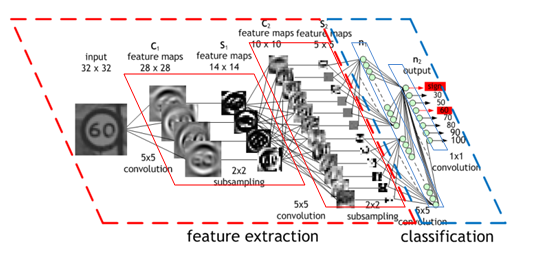
\includegraphics[scale=0.7]{convolutional_neural_network_structure} \]
  \centering
  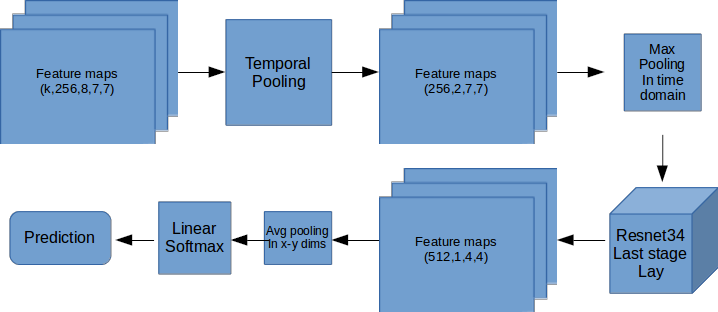
\includegraphics[scale=0.42]{mlp}
  \caption{\gr Η δομή του ταξινομητή \tl{MLP}}
  % \caption{\en Structure of the MLP classifier \gr}
  \label{fig:gr_mlp_structure}
\end{figure}
\gr
Σε προηγούμενες ενότητες χρησιμοποιήσαμε κλασσικούς ταξινομητές όπως τον Γραμμικό, έναν \en RNN \gr και έναν \en SVM\gr.
Τελευταίoi αλλά εξίσου σημαντικoi, μια άλλη ευρέως κατηγορία ταξινομητών είναι οι \en Multilayer Perceptron (MLP)\gr.
Σχεδιάζουμε έναν ταξινομητή \en MLP \gr όπως φαίνεται στο σχήμα \ref{fig:gr_mlp_structure} για διάρκεια δείγματος ίση με 8. H
λειτουργία του περιγράφεται κατωτέρω:

\begin{itemize}
\item Στην αρχή, μετά το \en 3D Roi Align \gr και για  διάρκεια του δείγματος ίση με  8 καρέ,
λαμβάνουμε ένα χάρτη ενεργοποίησης μεγέθους  $(k, 256, 8, 7, 7)$ όπου \tl{\textit{k}} είναι ο αριθμός των συνδεδεμένων ToIs. Εμπνευσμένοι
από προηγούμενες ενότητες, εκτελούμε \en temporal pooling \gr ακολουθούμενο  από
\en max pooling \gr  στην  διάσταση της διάρκειας του δείγματος. Έτσι, έχουμε τώρα έναν χάρτη χαρακτηριστικών 
με διαστάσεις ίσες με (2, 256, 7, 7), τις οποίες αναδιαμορφώνουμε σε
(256, 2, 7, 7) και τροφοδοτούμε σε \en layers \gr που εξήχθησαν από το τελευταίο στάδιο του \en ResNet34\gr.
Αυτά τα στάδια περιλαμβάνουν 3 \en Residual Layers \gr  με \en stride \gr  ίσο με 2 σε όλες τις 3
διαστάσεις και αριθμό εξόδου φίλτρων ίσου με 512.
\item Μετά τα \en Residual Layers\gr, κάνουμε \en avg pooling \gr για τις διαστάσεις \en \textit{ x-y}\gr.
Έτσι, έχουμε ως  εξόδο, χάρτες ενεργοποίησης με μέγεθος διαστάσεων ίσο με (512,).
Τέλος, τροφοδοτούμε  αυτoύς  τους  χαρακτηριστικούς  χάρτες σε ένα γραμμικό \en layer \gr προκειμένου να εξάγουμε την κλάση
του υποψήφιου \en action tube, \gr μετά την εφαρμογή της λειτουργίας \en  Soft-Max\gr.
\end{itemize}

\subsection{Κλασσικό \en training}
Όπως προαναφέρθηκε προηγουμένως, ο κώδικας εκπαίδευσης απαιτεί την εκτέλεση ενός μόνο βίντεο ανά \en GPU\gr, επειδή τα βίντεο έχουν διαφορετική διάρκεια το καθένα.
Για προηγούμενες προσεγγίσεις, μας ήρθε η  ιδέα του προϋπολογισμού των χαρακτηριστικά των \en action tubes \gr του βίντεο και στη συνέχεια
εκπαιδεύουμε μόνο τον ταξινομητή. Ωστόσο, για αυτό το βήμα, εκπαιδεύσαμε τον ταξινομητή μας με τον κλασικό τρόπο για να λάβουμε
αποτελέσματα ταξινόμησης. Φυσικά, χρησιμοποιήσαμε ένα προεκπαιδευμένο \en TPN\gr, του οποίου τα \en layers \gr παγώσαμε  για να μην εκπαιδευτούν.
Προσπαθήσαμε να εξερευνήσουμε διαφορετικές αναλογίες μεταξύ του αριθμού των \en action tubes \gr προσκηνίου και του συνολικού αριθμού των
\en action tubes \gr ανά βίντεο. Οι πρώτες 3 προσομοιώσεις περιλαμβάνουν σταθερό αριθμό συνολικών \en action tubes \gr και μεταβλητή αναλογία
μεταξύ του αριθμού των \en action tubes \gr προσκηνίου και φόντου. Αρχίσαμε χρησιμοπιώντας μόνο \en action tubes \gr προσκηνίου, το  οποίο
σημαίνει ότι 32 από τα 32  \en action tubes  \gr είναι προσκηνίου, μετά τα μισά από τα προτεινόμενα  \en action tubes, \gr δηλαδή 16 από 32 και
τέλος λιγότερο από το ήμισυ, δηλαδή 14 από τα 32.
Μετά από αυτό, πειραματιζόμαστε χρησιμοποιώντας έναν σταθερό αριθμό \en action tubes \gr προσκηνίου και μεταβλητού αριθμού συνολικών \en action tubes, \gr o oποίος είναι 16, 24 και 32. Τα αποτελέσματα των επιδόσεων παρουσιάζονται στον πίνακα \ref{table:gr_mlp_reg}.

\begin{center}
  \en
  \begin{longtable}{|| c | c || c c c ||}
    \hline
    \multirow{2}{*}{\textbf{FG tubes}} & \multirow{2}{*}{\textbf{Total tubes}} & {} &  \textbf{mAP} & {} \\
    {} & {} & 0.5 & 0.4 & 0.3 \\
    \hline
    32 & \multirow{3}{*}{32} &1.28 & 1.73 & 1.87  \\
    \cline{1-1} \cline{3-5}
    16 & {} & 3.98 & 4.38 & 4.38  \\
    \cline{1-1} \cline{3-5}
    14 & {} & 0.40 & 0.40 & 0.40 \\
    \hline
    \multirow{3}{*}{8} & 16 & 9.41 & 12.59 & 14.61 \\
    \cline{2-5}
    {} & 24 & 12.32 & 15.53 & 18.57 \\
    \cline{2-5}
    {} & 32 & 7.16 & 10.92 & 13.00 \\
    \hline
    \caption{\gr Η \tl{mAP} επίδοση του ταξινομητή \tl{MLP} για την κλασσική διαδικασία εκπαίδευσης}
    % \caption{\en MLP's mAP performance for regular training procedure\gr }
    \label{table:gr_mlp_reg}
  \end{longtable}
\end{center}

\newpage

Τα αποτελέσματα δείχνουν ότι  οι πρώτες 3 προσεγγίσεις μας δίνουν πολύ άσχημα αποτελέσματα.
Συγκρίνοντας τες με τις υπόλοιπους 3, ήρθαμε με το συμπέρασμα ότι χρειαζόμαστε
το πολύ 8 \en action tubes \gr προσκηνίου, ακόμη και όταν ο λόγος μεταξύ του αριθμού \en action tubes \gr
του προσκηνίου και του φόντου είναι υπέρ του δεύτερου. Πιθανότατα, πάρα πολλά
\en action tubes \gr προσκηνίου κάνουν την αρχιτεκτονική μας να έρθει σε κατάσταση \en overfitting \gr και
συνεπώς να είναι ανίκανη να γενικεύει.

\subsection{Εξαγωγή χαρακτηριστικών}

Όπως αναφέρθηκε προηγουμένως, εκπαιδεύσαμε τον ταξινομητή \en MLP \gr χρησιμοποιώντας προ-υπολογισμένους
χάρτες χαρακτηριστικών. Αυτοί οι χάρτες περιλαμβάνουν τόσο \en action tubes \gr που είναι στο  προσκήνιο όσο και στο  φόντο. Με
βάση τα συμπεράσματα που προέκυψαν  στα προηγούμενα μέρη, θα εκπαιδεύσουμε τον \tl{MLP} 
μόνο για  αριθμό \en action tubes \gr προσκηνίου ίσο με 4 και 8. Επιπλέον
Θα  εκπαιδεύσουμε τον ταξινομητή μας για 3 διαφορετικές αναλογίες, οι οποίες είναι 1:1, 1:2 και 1:3.
Ο πίνακας \ref{table:gr_mlp_extract_jhdmb} δείχνει αυτές τις περιπτώσεςι καθώς 
και τις αντίστοιχες επιδόσεις του \en mAP, \gr κατά τη διάρκεια του βήματος επικύρωσης.
\begin{center}
  \en
  \begin{longtable}{|| c | c || c c c ||}
    \hline
    \multirow{2}{*}{\textbf{FG tubes}} & \multirow{2}{*}{\textbf{Total tubes}} & {} & \textbf{mAP} & {} \\
    {} & {} & 0.5 & 0.4 & 0.3 \\
    \hline
    \multirow{3}{*}{4} & 6 & 4,37 & 8,54 & 10,12 \\
    \cline{2-5}
    {} & 8 & 5.89 & 9.54 & 13.61 \\
    \cline{2-5}
    {} & 12 & 9.51 & 12.8 & 14.6  \\
    \cline{2-5}
    {} & 16 & 6.80 & 13.17 & 14.67 \\
    \hline
    \multirow{4}{*}{8} & 12 & 8,62 & 12,32 & 14,74 \\
    \cline{2-5}
    {} & 16 & 8.49 & 13.94 & 15.09 \\
    \cline{2-5}
    {} & 24 & 6.72 & 12.17 & 15.30 \\
    \cline{2-5}
    {} & 32 & 13.27 & 17.64 & 18.97 \\
    \hline

    \caption{\gr Τα αποτελέσματα του \tl{mAP} για τον ταξινομητή \tl{MLP} εκπαιδεύοντας τον
      χρησιμοποιώντας \tl{pre-extracted features}}
  % \caption{\en mAP results for MLP trained using extracted features\gr }
  \label{table:gr_mlp_extract_jhdmb}
\end{longtable}
\end{center}

Συγκρίνοντας τα αποτελέσματα από τους πίνακες \ref{table:gr_mlp_extract_jhdmb}  και \ref{table:gr_mlp_reg}, είναι σαφές ότι χρειαζόμαστε 8
\en tubes \gr προσκηνίου για να λειτουργεί καλά ο ταξινομητής \en MLP. \gr  Ωστόσο, δεν είναι πολύ σαφές ποια από
τις  δύο προτεινόμενες εκπαιδευτικές διαδικασίες είναι καλύτερη, αλλά αν πρέπει να αποφασίσουμε μία
μέθοδο, θα επιλέξουμε τη χρήση προϋπολογισμένων χαρακτηριστικών. Η προσέγγιση αυτή
κατορθώνει να επιτύχει τα καλύτερα αποτελέσματα, και ειδικά όταν έχουμε 8
\en tubes \gr προσκηνίου και 32 συνολικά. Επίσης, συγκρίνοντας τις μεθόδους με 4 ή 8 θετικά
\en action tubes\gr, είναι σαφές ότι θα προτιμούσαμε να χρησιμοποιούμε 8 γενικά. Ωστόσο, δεν είναι
σαφές ποια αναλογία είναι καλύτερη, επειδή, έχουμε καλύτερα αποτελέσματα όταν έχουμε 8
\en action tubes \gr και αναλογία 1:4 ενώ έχουμε καλύτερα αποτελέσματα όταν η αναλογία είναι 1:3
με 4 \en action tubes.\gr


% \end{document}